%# -*- coding: utf-8-unix -*-
\chapter{双图决策树对消项说明}
\label{app:cancel}

本附录介绍了两种类型的符号化对消项,并介绍了其在GPDD这种符号化构造方法中的特性,并介绍了对消项的存在对电路简化中影响。

\section{符号化对消项概念介绍}
\label{sec:cancel:intro}

我们知道构造符号化表达式的过程中,我们会将没有可以互相抵消的项约去,以得到最简洁的电路表达式。
这样有利于电路分析,抛开无关紧要的项,同时也减少了运算过程中的复杂度,减少了不必要的数值误差。
符号化对消项主要有两类:加性对消项和公因子对消项。
加性对消项指的是可以在符号化表达中正负抵消的项。
而公因子对消项指的是在符号化表达式中成为分子分母共同的因子可以相互抵消的项。比如,在如下所示的公式中:

\begin{equation}
H\left( s \right) = \frac{ab + bc - ab}{bd}
\end{equation}

这里$ab$和$-ab$为加性对消项,而这里的$b$也是公因子对消项。
加性对消项会在对符号化公式求值的过程中引入不必要的数值误差,而公因子对消项除了数值误差意外,也在我们进行符号化约减的过程中引入了困难。

过去过去大量的符号化方法中,都存在对消项的问题,由于大量冗余的符号化对消项的存在,大大降低了内存空间的使用效率,同时引入了本应在符号化计算过程中避免的数值计算误差。
之所以没有通过一些方法匹配得到符号化表达中的对消项,主要原因在于进行这种匹配时间复杂度非常得高,需要对所有的符号化项进行两两比较,基本不可行。
\parencite{GShi-GPDD-2013}中宣称,GPDD结构中不存在符号化对消项。
经笔者验证发现,GPDD当中的确不存在加性符号化对消项,但有可能出现公因子对消项。
下面针对这两种不同的对消项给出证明。

\section{双图决策树无加性对消项证明}
\label{sec:cancel:add}

我们知道GPDD中每一条从根节点出发,到达1结点的路径可以构造出一个符号化项,称这样的路径为$P$,由$P$构造得到的符号化项为$T_P$。
由于GPDD中每一层仅一个符号,且每个符号有且仅有两种在$P$中出现可能性(包含或不包含),故不同的路径$P$必然不同。
如果我们可以证明路径$P$和符号化项$\left|T_P\right|$(加上绝对值去除符号的影响)构成的两个集合一一对应,那么由于$P$两两不相同,且两个集合均为有限集合,那么$\left|T_P\right|$也必然两两不相同,从而不可能出现加性对消项。
那么证明GPDD中不存在加性对消项的任务就转变为了证明两种集合一一对应的问题。

考虑某个GPDD构造的符号表共有N个符号,分别为${\mathbf{S}} = \left\{ {{S_1},{S_2}, \cdots ,{S_N}} \right\}$。
一个符号化项$\left|T_P\right|$可以写作这样的形式。

\begin{equation}
\left| {{T_P}} \right| = \prod\limits_{i = 1}^N {S_i^{{\alpha _i}}}
\end{equation}

其中这里的$\alpha _i$可以由路径$P$的边的性质决定,如下所示。

\begin{equation}
{\alpha _i} = \left\{ {
	\begin{array}{*{20}{c}}
	1 & {{S_i}{\text{下连接的边在}P\text{中为实线}}}  \\
	0 & {{S_i}{\text{下连接的边在}P\text{中为虚线或不存在}}}  \\
	\end{array} } \right.
\end{equation}

这样,我们根据$T_P$的定义可以直接得到$P \rightarrow \left|T_P\right|$的映射关系,如果可以找到一种方法形成的$\left|T_P\right| \rightarrow P$映射,那么$P \leftrightarrow \left|T_P\right|$之间的一一映射则可完成。

假设路径$P$由这样的边集组成${\mathbf{E}} = \left\{ {{E_1},{E_2}, \cdots ,{E_N}} \right\}$。
其中$E_i$为元件$S_i$这个节点下连接的边。如$S_i$节点不存在,则忽略该$E_i$。
给出任意一个$T_P$,我们可以决定$P$的连接情况如下所示。

\begin{equation}
{E_i} = \left\{ {
	\begin{array}{*{20}{c}}
	{{S_i}{\text{下的实线}}} & {{\alpha _i} = 1}  \\
	{{S_i}{\text{下的虚线}}} & {{\alpha _i} = 0}  \\
	\end{array} } \right.
\end{equation}

故这样形成了$\left|T_P\right| \rightarrow P$的映射,故由$P$和$T_P$组成的两个集合之间一一映射。
故可以有以下定理。

\begin{thm}
	双图决策图结构中不存在加性对消项。
\end{thm}

从上述证明过程中,可以看到,不仅GPDD中不存在加性对消项,而且每个符号项前的系数仅为$\pm1$。

\section{双图决策树公因子对消项情况}
\label{sec:cancel:factor}

虽然,GPDD中不存在加性对消项,但是却有可能出现公因子对消项。
我们通过举反例的方式对这一点进行说明,并介绍其在电路简化过程中造成的问题。

\subsection{公因子对消项反例}
\label{subsec:cancel:factor:example}

我们考虑这样一个如图\ref{fig:CirCase}所示的两级电路。
但我们其实只观测第一级的电压响应,所以第二级所用的元件对第一级没有任何贡献。

\begin{figure}[!htp]
	\centering
	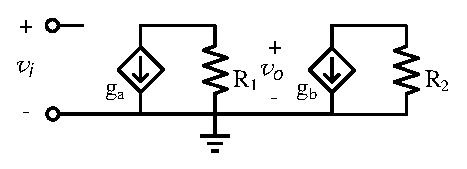
\includegraphics[width=0.48\textwidth]{app1/CirCase.eps}
	\bicaption[fig:CirCase]{存在公因子对消项的示例电路}{存在公因子对消项的示例电路}{Fig}{Circuit example with common factor}
\end{figure}

\begin{figure}[!htp]
	\centering
	\includegraphics[width=0.17\textwidth]{app1/GPDDCase.eps}
	\bicaption[fig:GPDDCase]{存在公因子对消项的示例电路}{存在公因子对消项的示例电路}{Fig}{Circuit example with common factor}
\end{figure}

但是可以在图\ref{fig:GPDDCase}中看到,其实其中第二级点元件$R_2$仍然存在于GPDD结构中。
根据这样的GPDD结构,经过计算,我们可以得到如下的电路传输函数:

\begin{equation}
H\left( s \right) =  - \frac{{{g_a}{G_2}}}{{{G_1}{G_2}}}
\end{equation}

可以看到这里$R_2$形成了符号化公因子对消项。
因为GPDD中所有到1结点的路径均经过$R_2$节点,并且$R_2$节点的右儿子均为零。

\subsection{对自动低阶模型生成中电路图约减过程的影响}
\label{subsec:cancel:factor:influence}

在图的约减过程中,根据图\ref{fig:GPDDCase}的情况下,如果我们考虑$R_2$的导纳为零,即断路情况。
根据我们计算有元件取极限值的算法,GPDD在$R_2$这个节点会选择右儿子节点的值,在这里即为$0$。
可以看到这导致整个GPDD结构中没有一条到1结点的路径,那么必然会在计算传输函数过程中,得到$0/0$的结果,从而造成了计算的错误。
如果将$R_2$短路即可避免这一情况。

这种情况如果在一开始元件关键性计算的过程就发生,那么会立刻归为\ref{subsubsec:simp:alg:special:sign}中的第一种特殊特殊情况。
如果是在发生了多个元件删去后的结果,那么就会成为\ref{subsubsec:simp:alg:special:reduce}中第二种特殊情况。